\documentclass{article}
\usepackage[margin=1in]{geometry}
\usepackage[linesnumbered,ruled,vlined]{algorithm2e}
\usepackage{amsfonts}
\usepackage{amsmath}
\usepackage{amssymb}
\usepackage{amsthm}
\usepackage{enumitem}
\usepackage{fancyhdr}
\usepackage{hyperref}
\usepackage{minted}
\usepackage{multicol}
\usepackage{pdfpages}
\usepackage{standalone}
\usepackage[many]{tcolorbox}
\usepackage{tikz-cd}
\usepackage{transparent}
\usepackage{xcolor}
% \tcbuselibrary{minted}

\author{Nathan Solomon}

\newcommand{\fig}[1]{
    \begin{center}
        \includegraphics[width=\textwidth]{#1}
    \end{center}
}

% Math commands
\renewcommand{\d}{\mathrm{d}}
\DeclareMathOperator{\id}{id}
\DeclareMathOperator{\im}{im}
\DeclareMathOperator{\proj}{proj}
\DeclareMathOperator{\Span}{span}
\DeclareMathOperator{\Tr}{Tr}
\DeclareMathOperator{\tr}{tr}
\DeclareMathOperator{\ad}{ad}
\DeclareMathOperator{\ord}{ord}
%%%%%%%%%%%%%%% \DeclareMathOperator{\sgn}{sgn}
\DeclareMathOperator{\Aut}{Aut}
\DeclareMathOperator{\Inn}{Inn}
\DeclareMathOperator{\Out}{Out}
\DeclareMathOperator{\stab}{stab}

\newcommand{\N}{\ensuremath{\mathbb{N}}}
\newcommand{\Z}{\ensuremath{\mathbb{Z}}}
\newcommand{\Q}{\ensuremath{\mathbb{Q}}}
\newcommand{\R}{\ensuremath{\mathbb{R}}}
\newcommand{\C}{\ensuremath{\mathbb{C}}}
\renewcommand{\H}{\ensuremath{\mathbb{H}}}
\newcommand{\F}{\ensuremath{\mathbb{F}}}

\newcommand{\E}{\ensuremath{\mathbb{E}}}
\renewcommand{\P}{\ensuremath{\mathbb{P}}}

\newcommand{\es}{\ensuremath{\varnothing}}
\newcommand{\inv}{\ensuremath{^{-1}}}
\newcommand{\eps}{\ensuremath{\varepsilon}}
\newcommand{\del}{\ensuremath{\partial}}
\renewcommand{\a}{\ensuremath{\alpha}}

\newcommand{\abs}[1]{\ensuremath{\left\lvert #1 \right\rvert}}
\newcommand{\norm}[1]{\ensuremath{\left\lVert #1\right\rVert}}
\newcommand{\mean}[1]{\ensuremath{\left\langle #1 \right\rangle}}
\newcommand{\floor}[1]{\ensuremath{\left\lfloor #1 \right\rfloor}}
\newcommand{\ceil}[1]{\ensuremath{\left\lceil #1 \right\rceil}}
\newcommand{\bra}[1]{\ensuremath{\left\langle #1 \right\rvert}}
\newcommand{\ket}[1]{\ensuremath{\left\lvert #1 \right\rangle}}
\newcommand{\braket}[2]{\ensuremath{\left.\left\langle #1\right\vert #2 \right\rangle}}

\newcommand{\catname}[1]{{\normalfont\textbf{#1}}}

\newcommand{\up}{\ensuremath{\uparrow}}
\newcommand{\down}{\ensuremath{\downarrow}}

% Custom environments
\newtheorem{thm}{Theorem}[section]

\definecolor{probBackgroundColor}{RGB}{250,240,240}
\definecolor{probAccentColor}{RGB}{140,40,0}
\newenvironment{prob}{
    \stepcounter{thm}
    \begin{tcolorbox}[
        boxrule=1pt,
        sharp corners,
        colback=probBackgroundColor,
        colframe=probAccentColor,
        borderline west={4pt}{0pt}{probAccentColor},
        breakable
    ]
    \color{probAccentColor}\textbf{Problem \thethm.} \color{black}
} {
    \end{tcolorbox}
}

\definecolor{exampleBackgroundColor}{RGB}{212,232,246}
\newenvironment{example}{
    \stepcounter{thm}
    \begin{tcolorbox}[
      boxrule=1pt,
      sharp corners,
      colback=exampleBackgroundColor,
      breakable
    ]
    \textbf{Example \thethm.}
} {
    \end{tcolorbox}
}

\definecolor{propBackgroundColor}{RGB}{255,245,220}
\definecolor{propAccentColor}{RGB}{150,100,0}
\newenvironment{prop}{
    \stepcounter{thm}
    \begin{tcolorbox}[
        boxrule=1pt,
        sharp corners,
        colback=propBackgroundColor,
        colframe=propAccentColor,
        breakable
    ]
    \color{propAccentColor}\textbf{Proposition \thethm. }\color{black}
} {
    \end{tcolorbox}
}

\definecolor{thmBackgroundColor}{RGB}{235,225,245}
\definecolor{thmAccentColor}{RGB}{50,0,100}
\renewenvironment{thm}{
    \stepcounter{thm}
    \begin{tcolorbox}[
        boxrule=1pt,
        sharp corners,
        colback=thmBackgroundColor,
        colframe=thmAccentColor,
        breakable
    ]
    \color{thmAccentColor}\textbf{Theorem \thethm. }\color{black}
} {
    \end{tcolorbox}
}

\definecolor{corBackgroundColor}{RGB}{240,250,250}
\definecolor{corAccentColor}{RGB}{50,100,100}
\newenvironment{cor}{
    \stepcounter{thm}
    \begin{tcolorbox}[
        enhanced,
        boxrule=0pt,
        frame hidden,
        sharp corners,
        colback=corBackgroundColor,
        borderline west={4pt}{0pt}{corAccentColor},
        breakable
    ]
    \color{corAccentColor}\textbf{Corollary \thethm. }\color{black}
} {
    \end{tcolorbox}
}

\definecolor{lemBackgroundColor}{RGB}{255,245,235}
\definecolor{lemAccentColor}{RGB}{250,125,0}
\newenvironment{lem}{
    \stepcounter{thm}
    \begin{tcolorbox}[
        enhanced,
        boxrule=0pt,
        frame hidden,
        sharp corners,
        colback=lemBackgroundColor,
        borderline west={4pt}{0pt}{lemAccentColor},
        breakable
    ]
    \color{lemAccentColor}\textbf{Lemma \thethm. }\color{black}
} {
    \end{tcolorbox}
}

\definecolor{proofBackgroundColor}{RGB}{255,255,255}
\definecolor{proofAccentColor}{RGB}{80,80,80}
\renewenvironment{proof}{
    \begin{tcolorbox}[
        enhanced,
        boxrule=1pt,
        sharp corners,
        colback=proofBackgroundColor,
        colframe=proofAccentColor,
        borderline west={4pt}{0pt}{proofAccentColor},
        breakable
    ]
    \color{proofAccentColor}\emph{\textbf{Proof. }}\color{black}
} {
    \qed \end{tcolorbox}
}

\definecolor{noteBackgroundColor}{RGB}{240,250,240}
\definecolor{noteAccentColor}{RGB}{30,130,30}
\newenvironment{note}{
    \begin{tcolorbox}[
        enhanced,
        boxrule=0pt,
        frame hidden,
        sharp corners,
        colback=noteBackgroundColor,
        borderline west={4pt}{0pt}{noteAccentColor},
        breakable
    ]
    \color{noteAccentColor}\textbf{Note. }\color{black}
} {
    \end{tcolorbox}
}


\fancyhf{}
\setlength{\headheight}{24pt}

\date{\today}
\title{Math 151A Homework \#7}

\begin{document}
\maketitle

\begin{prob}
\end{prob}
\begin{enumerate}[label=(\alph*)]
    \item Let $f(x) = x^2 e^{-x}$. Then
        \begin{align*}
            \int_0^1 f(x) \d x &= \frac{f(0)+f(1)}{2} \\
                               &= \frac{0}{2} + \frac{1^2}{2e} \\
                               &= \frac{1}{2e} \\
                               &\approx 0.1839
        \end{align*}
        This is fairly close to the actual answer, which is $2-5/e\approx 0.1606$
    \item Let $f(x) = 2x/(x^2-4)$. Then
        \begin{align*}
            \int_1^{1.6} f(x) \d x &= (1.6-1) \frac{f(1)+f(1.6)}{2} \\
                                   &= 0.3 \left( \frac{2}{1-4} + \frac{3.2}{2.56-4} \right) \\
                                   &= 0.3 \left( -\frac{2}{3} - \frac{20}{9} \right) \\
                                   &= -0.2 - \frac{2}{3} \\
                                   &= -0.8666\dots
        \end{align*}
        The actual answer is $-0.7340\dots$ which is not too far off.
\end{enumerate}


\bigskip
\begin{prob}
\end{prob}
The trapezoidal rule says
\[ 2 \cdot \frac{f(0)+f(2)}{2} = 4, \]
and Simpson's rule says that
\[ \frac{1}{3} \cdot \left( f(0)+4f(1)+f(2) \right) = 2, \]
so $(1/3)(4+4f(1))=2$, which means $4(1+f(1))=6$, so
\[ f(1)=- \frac{1}{2}. \]


\bigskip
\begin{prob}
\end{prob}
The actual value of the integral is \begin{align*}
    \int_1^2 x \ln (x) \d x &= \left[ \frac{x^2}{2} \ln(x) \right]_1^2 - \int_1^2 \frac{x^2}{2} \cdot \frac{1}{x }\d x \\
                            &= 2 \ln(2) - \frac{1}{2} \ln(1) - \left[ \frac{x^2}{4} \right]_1^2 \\
                            &= 2 \ln(2) - \frac{3}{4} \\
                            &\approx 0.636294
\end{align*}
The composite trapezoidal rule gives $0.639900$ (relative error of $0.00566737$), and the composite Simpson's rule gives $0.636310$ (relative error of $0.0000243106$). Here is the code I used to calculate those:
\par
\begin{lstlisting}[language=Python]
>>> from math import log
>>> def f(x): return x * log(x)
... 
>>> x_i = [1, 1.25, 1.5, 1.75, 2]
>>> w_i = [.125, .25, .25, .25, .125]
>>> sum([f(x_i[i]) * w_i[i] for i in range(5)])
0.639900477687986
>>> w_i = [1/12, 1/3, 1/6, 1/3, 1/12]
>>> sum([f(x_i[i]) * w_i[i] for i in range(5)])
0.6363098297969493
\end{lstlisting}

\bigskip
\begin{prob}
\end{prob}
We already know that the error for Simpson's rule is
\[ E[f] = \sum_{j=1}^{n/2} \frac{h^5f^{(4)}(\xi_j)}{90}, \]
where each $\xi_j$ is in $[a,b]$, and $nh=b-a$. By IVT, there is some $\xi \in [a,b]$ such that
\[ \sum_{j=1}^{n/2} f^{(4)}(\xi_j) = \frac{n}{2} f^{(4)}(\xi), \]
so the error is
\[ E[f] = \frac{h^4(b-a)}{180} f^{(4)}(\xi), \]
and the absolute error is the absolute value of that. Also, the given inequality is true by the triangle inequality.

\bigskip
\begin{prob}
\end{prob}
\begin{enumerate}[label=(\alph*)]
    \item If $f(x)=x \ln(x)$, then $f'(x) = \ln(x)+1$, and $f''(x) = \frac{1}{x}$. Note that the domain of $f$ is the set of positive real numbers, so the lowest posible upper bound for $f''(\mu)$ when $\mu \in (a,b)$ is $1/a$ (assuming $a < b$). This means the absolute error is guaranteed to be less than $h^2(b-a)/(12a)$. If $a=1$ and $b=2$ and we want to guarantee that the absolute error is less than $\tau = 10^{-5}$, we need \begin{align*}
            \frac{h^2}{12} &< \tau = 10^{-5} \\
            h &< \sqrt{1.2 \times 10^{-4}} \approx 0.010954 \\
            n = \frac{1}{h} &> 91.287 \\
            n &\geq 92.
    \end{align*}
\item With the composite Simpson's rule, the absolute error is
    \[ E[f] = \frac{h^4(b-a)}{180} \abs{f^{(4)}(\xi)} \]
    for some $\xi \in [a,b]$. We have the same $f,a,b$ as before, so $f'''(x) = -1/x^2$ and $f^{(4)}(x)=2/x^3$, meaning the upper bound on $\abs{f^{(4)}(\xi)}$ is $2/a^3=2$. Therefore \begin{align*}
        E[f] \leq \frac{h^4(b-a)}{180} \cdot 2 &< \tau = 10^{-5} \\
        h^4 &< 9 \times 10^{-4} \\
        h &< \sqrt[4]{9 \times 10^{-4}} \approx 0.1732 \\
        n = \frac{1}{h} &> 5.7735 \\
        n &\geq 6.
    \end{align*}
\end{enumerate}


\bigskip
\begin{prob}
\end{prob}
This is equivalent to ensuring that whenever $f$ is a degree 3 polynomial,
the error for that quadrature rule is zero. If $f(x)=\alpha +\beta x + \gamma x^2 + \delta x^3$, then we have the following equations: \begin{align*}
    f'(x) &= \beta + 2 \gamma x + 3 \delta x^2 \\
    I := \int_{-1}^1 f(x) \d x &= \left[ \alpha x + \frac{\beta x^2}{2} + \frac{\gamma x^3}{3} + \frac{\delta x^4}{4} \right]_{-1}^1 \\
    I &= \left( \alpha + \frac{\beta}{2} + \frac{\gamma}{3} + \frac{\delta}{4} \right) - \left( -\alpha + \frac{\beta}{2} - \frac{\gamma}{3} + \frac{\delta}{4} \right) \\
    I &= 2\alpha + \frac{2\gamma}{3} \\
    f(-1) &= \alpha - \beta + \gamma - \delta \\
    f(1) &= \alpha + \beta + \gamma + \delta \\
    f'(-1) &= \beta - 2 \gamma + 3 \delta \\
    f'(1) &= \beta + 2 \gamma + 3 \delta \\
    I &= a f(-1) + b f(1) + c f'(-1) + d f'(1) \\
    \begin{bmatrix}
        2 \\
        0 \\
        \frac{2}{3} \\
        0
    \end{bmatrix} &= \begin{bmatrix}
    1 & 1 & 0 & 0 \\
    -1 & 1 & 1 & 1 \\
    1 & 1 & -2 & 2 \\
    -1 & 1 & 3 & 3
    \end{bmatrix} \begin{bmatrix}
        a \\
        b \\
        c \\
        d
    \end{bmatrix} \\
    \begin{bmatrix}
        a \\
        b \\
        c \\
        d
    \end{bmatrix} &= \frac{1}{4} \begin{bmatrix}
    2 & -3 & 0 & 1 \\
    2 & 3 & 0 & -1 \\
    1 & -1 & -1 & 1 \\
    -1 & -1 & 1 & 1
    \end{bmatrix} \begin{bmatrix}
    2 \\
    0 \\
    \frac{2}{3} \\
    0
    \end{bmatrix} \\
    a &= 1 \\
    b &= 1 \\
    c &= \frac{1}{3} \\
    d &= - \frac{1}{3}.
\end{align*}

\bigskip
\begin{prob}
\end{prob}
\begin{enumerate}[label=(\alph*)]
    \item Given some initial guess $x_0$ for a solution to the equation, Newton's method says to iteratively apply \begin{align*}
            x_{n+1} &= x_n - \frac{f(x_n)}{f'(x_n)} \\
                    &= x_n - \sqrt{2\pi} \cdot e^{x_n^2/2} \cdot f(x_n).
    \end{align*}
\item The composite trapezoidal rule approximates $f(x)$ as \begin{align*}
        f(x) &= \frac{1}{\sqrt{2\pi}} \int_0^x e^{-t^2/2} \d t - 0.45 \\
             &= (-0.45) + \frac{1}{\sqrt{2\pi}} \sum_{j=1}^N \frac{x}{2N} \left( \exp \left( - \frac{((j-1)x/N)^2}{2} \right) + \exp \left( - \frac{(jx/N)^2}{2} \right) \right).
\end{align*}
Plugging that back in to Newton's method gives
\[ x_{n+1} = x_n + \exp\left( \frac{x_n^2}{2} \right) \left( 0.45 \sqrt{2\pi} - \frac{x}{2N} \sum_{j=1}^N \left[ \exp \left( - \frac{((j-1)x_n/N)^2}{2} \right) + \exp \left( - \frac{(jx_n/N)^2}{2} \right) \right] \right). \]

    \item When I use $N=50$ and $x_0=0.5$, the first guess to reach the desired tolerance is $x_4 = 1.644962$, but if I keep iterating, the method converges to $x\approx1.645002$. However, when I use $N=200$ (and $x_0=0.5$), it converges to $1.644863$ instead, and if I reduce $N$ to $20$, it converges to $1.645782$. We can assume that the higher $N$ is, the closer we get to the actual root.
        \begin{lstlisting}[language=Python]
#!/usr/bin/env python3
from math import exp, sqrt, pi

x = 0.5
N = 50
def f(x):
    summation = 0
    for j in range(N):
        summation += exp(0 - (j    *x/N)**2 / 2)
        summation += exp(0 - ((j+1)*x/N)**2 / 2)
    return -0.45 + summation * x / (2 * N * sqrt(2 * pi))

for i in range(100):
    print(f"x_{i} = {x}")
    residual = f(x)
    if abs(residual) < 1e-15:
        break
    x -= sqrt(2 * pi) * exp(x**2 / 2) * residual


x_0 = 0.5
x_1 = 1.234349525548872
x_2 = 1.5487272386153916
x_3 = 1.6380320881922388
x_4 = 1.6449621080925367
        \end{lstlisting}
\end{enumerate}

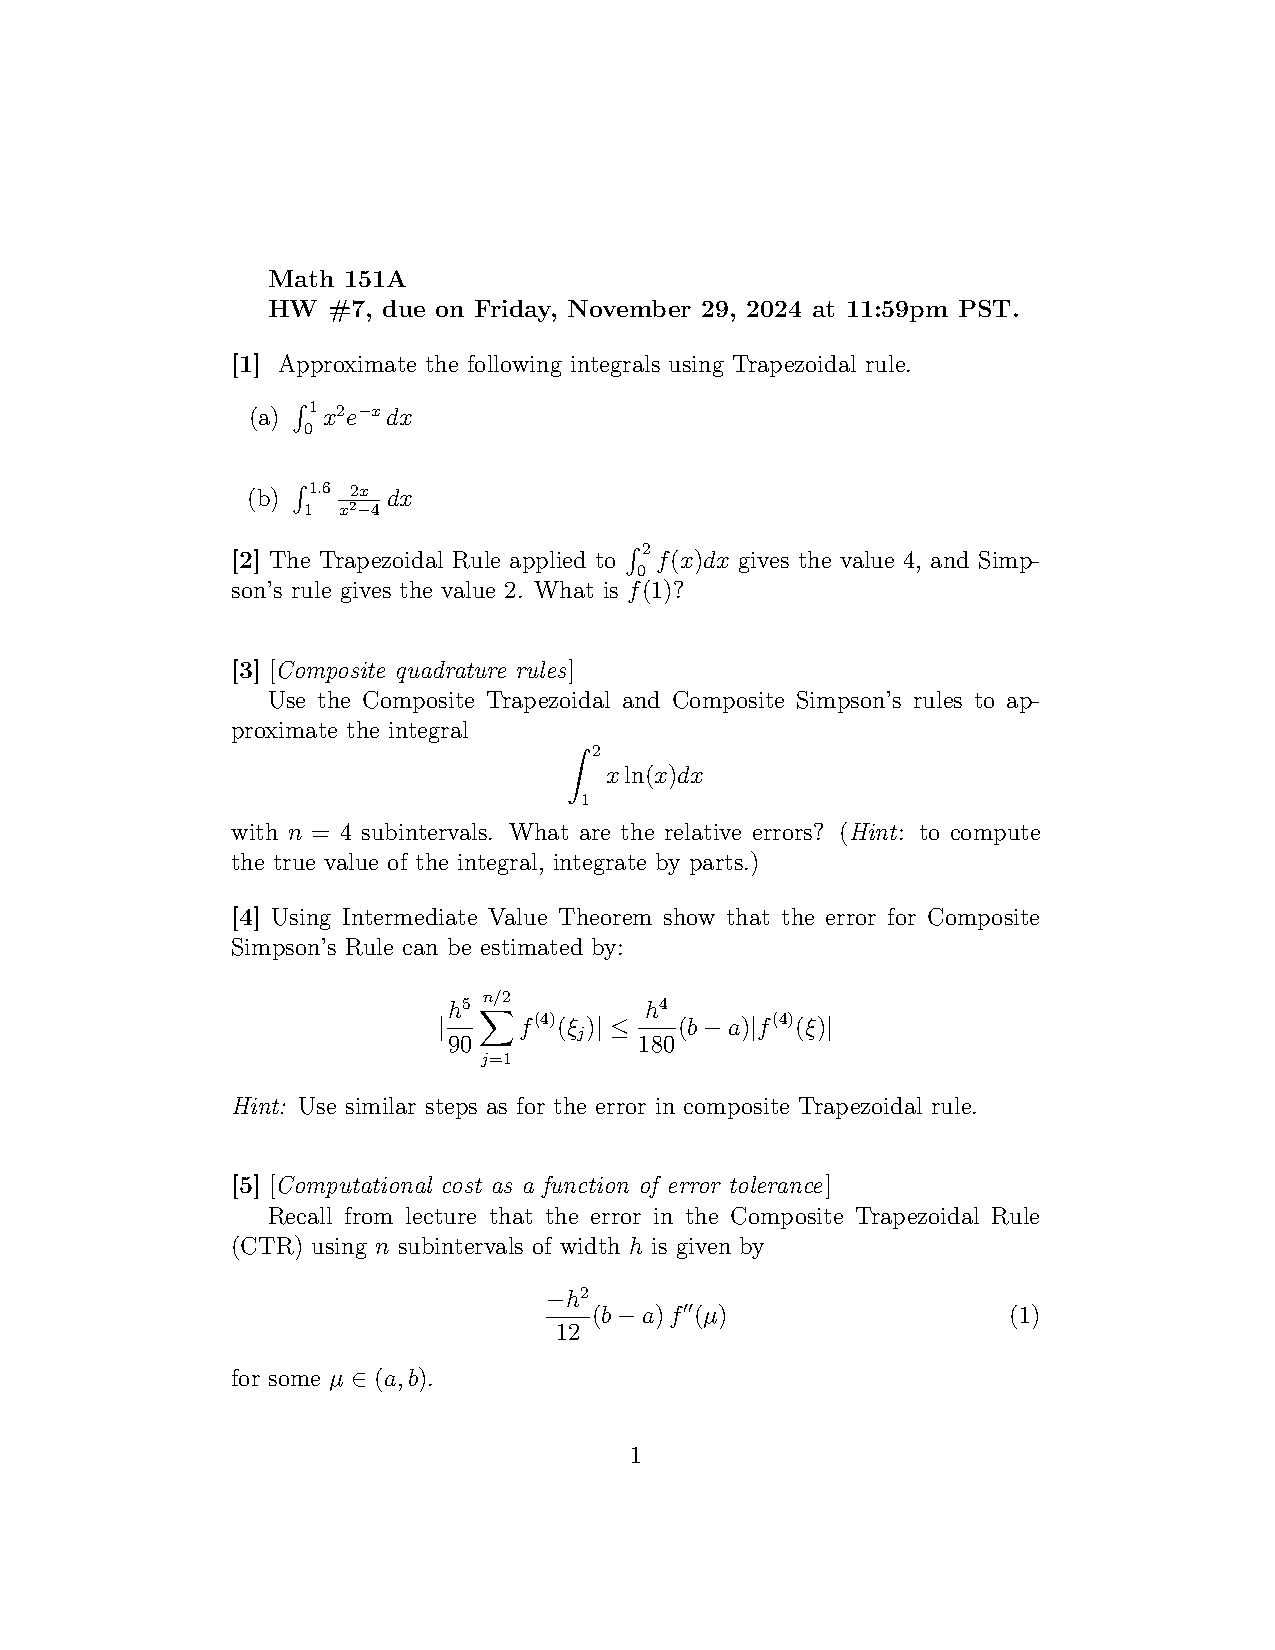
\includepdf[pages=-]{assignment.pdf}

\end{document}
